\documentclass[aspectratio=169]{beamer}
\usetheme{Madrid}
\usecolortheme{default}

\usepackage{tikz}
\usepackage{listings}
\usepackage{xcolor}
\usepackage{booktabs}
\usepackage{multicol}

\usetikzlibrary{shapes,arrows,positioning,fit,backgrounds}

% Listings configuration for Java
\lstset{
    language=Java,
    basicstyle=\ttfamily\footnotesize,
    keywordstyle=\color{blue}\bfseries,
    commentstyle=\color{green!60!black},
    stringstyle=\color{red},
    numbers=left,
    numberstyle=\tiny\color{gray},
    breaklines=true,
    frame=single,
    showstringspaces=false
}

\title{Week 10: Design Patterns\\Factory Method \& Object Pool}
\subtitle{OOP Course - Game Development Series}
\author{Instructor}
\date{\today}

\begin{document}

% =====================================================
% TITLE SLIDE
% =====================================================
\begin{frame}
    \titlepage
\end{frame}

% =====================================================
% TABLE OF CONTENTS
% =====================================================
\begin{frame}{Agenda}
    \tableofcontents
\end{frame}

% =====================================================
% SECTION 1: INTRODUCTION
% =====================================================
\section{Introduction}

\begin{frame}{Week 10 Overview}
    \begin{block}{Learning Journey}
        \textbf{Week 9}: Foundational patterns (Game Loop, Singleton)\\
        \textbf{Week 10}: Creational \& Performance patterns
    \end{block}

    \begin{columns}[T]
        \begin{column}{0.48\textwidth}
            \textbf{Factory Method Pattern}
            \begin{itemize}
                \item Problem: Hard-coded creation
                \item Solution: Polymorphic factories
                \item Benefit: Open/Closed Principle
            \end{itemize}
        \end{column}
        \begin{column}{0.48\textwidth}
            \textbf{Object Pool Pattern}
            \begin{itemize}
                \item Problem: GC pressure
                \item Solution: Object reuse
                \item Benefit: Stable performance
            \end{itemize}
        \end{column}
    \end{columns}

    \vspace{0.5cm}
    \begin{alertblock}{Four Branches}
        10-01 $\rightarrow$ 10-02 $\rightarrow$ 10-03 $\rightarrow$ 10-04 (Problem $\rightarrow$ Solution $\rightarrow$ Problem $\rightarrow$ Solution)
    \end{alertblock}
\end{frame}

\begin{frame}{What We'll Build}
    \textbf{Dungeon Escape Game Features:}
    \begin{multicols}{2}
        \begin{itemize}
            \item Dynamic obstacle spawning
            \item Three obstacle types (Spike, Goblin, Wolf)
            \item Collision detection
            \item Performance monitoring
            \item Safe spawning algorithm
        \end{itemize}
    \end{multicols}
\end{frame}

% =====================================================
% SECTION 2: BRANCH 10-01 - HARD-CODED CREATION
% =====================================================
\section{Branch 10-01: Hard-Coded Creation (Problem)}

\begin{frame}{10-01: The Problem}
    \begin{alertblock}{Hard-Coded Object Creation}
        WorldController directly creates concrete obstacle types using switch statement
    \end{alertblock}

    \begin{lstlisting}[basicstyle=\ttfamily\tiny]
// WorldController.java (Branch 10-01)
private void spawnRandomObstacle() {
    int type = random.nextInt(3);  // 0, 1, or 2
    Obstacle obstacle = null;

    switch (type) {
        case 0: obstacle = new Spike(x, y); break;   // Hard-coded!
        case 1: obstacle = new Goblin(x, y); break;  // Hard-coded!
        case 2: obstacle = new Wolf(x, y); break;    // Hard-coded!
    }

    activeObstacles.add(obstacle);
}
    \end{lstlisting}

    \textcolor{red}{\textbf{Problems identified on next slide...}}
\end{frame}

\begin{frame}{10-01: Why This is Bad}
    \begin{columns}[T]
        \begin{column}{0.48\textwidth}
            \textbf{\textcolor{red}{Problems:}}
            \begin{enumerate}
                \item \textbf{Tight Coupling}
                \begin{itemize}
                    \item WorldController depends on Spike, Goblin, Wolf classes
                    \item Cannot change without modifying WorldController
                \end{itemize}
                \item \textbf{Violates Open/Closed Principle}
                \begin{itemize}
                    \item Must modify existing code to add new type
                    \item Risky: might break existing functionality
                \end{itemize}
            \end{enumerate}
        \end{column}
        \begin{column}{0.48\textwidth}
            \begin{enumerate}
                \setcounter{enumi}{2}
                \item \textbf{Extensibility Issues}
                \begin{itemize}
                    \item Adding Dragon requires modifying switch
                    \item case 3: new Dragon(x, y);
                \end{itemize}
                \item \textbf{Merge Conflicts}
                \begin{itemize}
                    \item All developers edit same file
                    \item High risk of conflicts in switch statement
                \end{itemize}
            \end{enumerate}
        \end{column}
    \end{columns}

    \vspace{0.3cm}
    \begin{exampleblock}{Real-World Scenario}
        Team of 3 students: Alice adds Dragon, Bob adds Trap, Charlie adds Boss.\\
        All modify same switch statement $\rightarrow$ \textcolor{red}{MERGE CONFLICT!}
    \end{exampleblock}
\end{frame}

\begin{frame}{10-01: Dependency Diagram}
    \begin{center}
        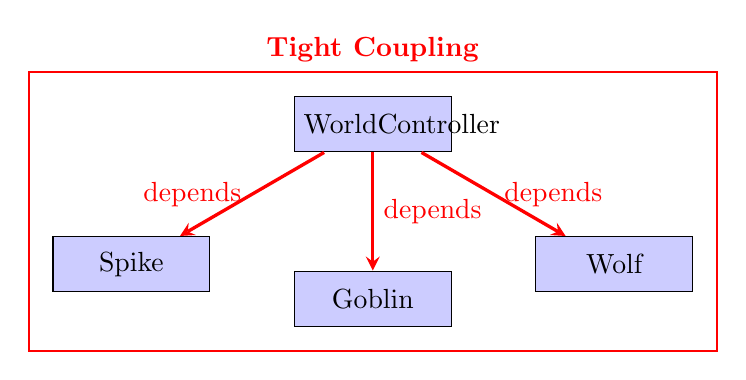
\begin{tikzpicture}[node distance=1.5cm]
            \tikzstyle{class} = [rectangle, draw, fill=blue!20, text width=5em, text centered, minimum height=2em]
            \tikzstyle{arrow} = [thick,->,>=stealth]

            \node [class] (wc) at (0,0) {WorldController};
            \node [class, below left=of wc] (spike) {Spike};
            \node [class, below=of wc] (goblin) {Goblin};
            \node [class, below right=of wc] (wolf) {Wolf};

            \draw [arrow, red, very thick] (wc) -- (spike) node[midway, left] {\textcolor{red}{depends}};
            \draw [arrow, red, very thick] (wc) -- (goblin) node[midway, right] {\textcolor{red}{depends}};
            \draw [arrow, red, very thick] (wc) -- (wolf) node[midway, right] {\textcolor{red}{depends}};

            \node [draw=red, thick, fit=(wc) (spike) (goblin) (wolf), inner sep=0.3cm, label=above:{\textcolor{red}{\textbf{Tight Coupling}}}] {};
        \end{tikzpicture}
    \end{center}

    \textbf{Problem:} WorldController must know about ALL concrete obstacle types!
\end{frame}

% =====================================================
% SECTION 3: BRANCH 10-02 - FACTORY METHOD
% =====================================================
\section{Branch 10-02: Factory Method Pattern (Solution)}

\begin{frame}{10-02: Factory Method Pattern}
    \begin{block}{Pattern Definition}
        \textbf{Intent:} Define an interface for creating objects, but let subclasses decide which class to instantiate.
    \end{block}

    \textbf{Key Idea:} Separate \textit{what} to create from \textit{how} to create it.

    \begin{columns}[T]
        \begin{column}{0.48\textwidth}
            \textbf{Before (10-01):}
            \begin{itemize}
                \item WorldController creates obstacles
                \item Uses switch statement
                \item Tight coupling to concrete types
            \end{itemize}
        \end{column}
        \begin{column}{0.48\textwidth}
            \textbf{After (10-02):}
            \begin{itemize}
                \item Factories create obstacles
                \item Polymorphic creation
                \item Loose coupling (interface only)
            \end{itemize}
        \end{column}
    \end{columns}
\end{frame}

\begin{frame}[fragile]{10-02: Factory Interface}
    \begin{lstlisting}[basicstyle=\ttfamily\scriptsize]
// ObstacleFactory.java
public interface ObstacleFactory {
    /**
     * Create an obstacle at the specified position
     * @param x X coordinate
     * @param y Y coordinate
     * @return Created obstacle instance
     */
    Obstacle createObstacle(int x, int y);
}
    \end{lstlisting}

    \textbf{Why interface?}
    \begin{itemize}
        \item Defines \textit{contract} for all factories
        \item Client (WorldController) depends on abstraction, not concrete classes
        \item Enables polymorphism: any factory can be used interchangeably
    \end{itemize}
\end{frame}

\begin{frame}[fragile]{10-02: Concrete Factories}
    \begin{columns}[T]
        \begin{column}{0.48\textwidth}
            \begin{lstlisting}[basicstyle=\ttfamily\tiny]
// SpikeFactory.java
public class SpikeFactory
    implements ObstacleFactory {

    @Override
    public Obstacle createObstacle(
        int x, int y) {
        return new Spike(x, y);
    }
}
            \end{lstlisting}

            \begin{lstlisting}[basicstyle=\ttfamily\tiny]
// GoblinFactory.java
public class GoblinFactory
    implements ObstacleFactory {

    @Override
    public Obstacle createObstacle(
        int x, int y) {
        return new Goblin(x, y);
    }
}
            \end{lstlisting}
        \end{column}
        \begin{column}{0.48\textwidth}
            \begin{lstlisting}[basicstyle=\ttfamily\tiny]
// WolfFactory.java
public class WolfFactory
    implements ObstacleFactory {

    @Override
    public Obstacle createObstacle(
        int x, int y) {
        return new Wolf(x, y);
    }
}
            \end{lstlisting}

            \vspace{0.3cm}
            \textbf{Key Points:}
            \begin{itemize}
                \item Each factory knows HOW to create its type
                \item Simple implementation (just return new)
                \item Can add complex initialization logic here
            \end{itemize}
        \end{column}
    \end{columns}
\end{frame}

\begin{frame}[fragile]{10-02: Client Usage}
    \begin{lstlisting}[basicstyle=\ttfamily\scriptsize]
// WorldController.java (Branch 10-02)
public class WorldController {
    private List<ObstacleFactory> factories;  // List of factories!

    public WorldController(NPC npc) {
        // Register all factories
        this.factories = Arrays.asList(
            new SpikeFactory(),
            new GoblinFactory(),
            new WolfFactory()
            // Easy to add: new DragonFactory()
        );
    }

    private void spawnRandomObstacle() {
        // Select random factory
        ObstacleFactory factory = factories.get(random.nextInt(factories.size()));

        // Create obstacle (polymorphic!)
        Obstacle obstacle = factory.createObstacle(x, y);
        activeObstacles.add(obstacle);
    }
}
    \end{lstlisting}

    \textcolor{green}{\textbf{No switch statement! Clean code!}}
\end{frame}

\begin{frame}{10-02: Architecture Diagram}
    \begin{center}
        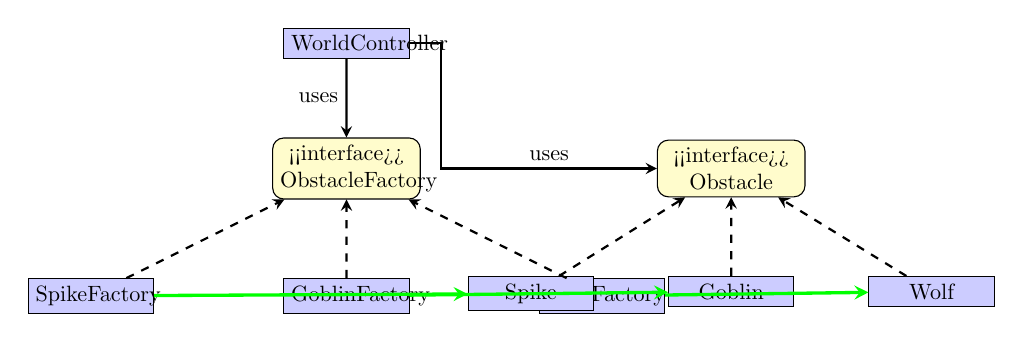
\begin{tikzpicture}[node distance=1.5cm, scale=0.8, every node/.style={scale=0.8}]
            \tikzstyle{interface} = [rectangle, draw, fill=yellow!20, text width=6em, text centered, rounded corners]
            \tikzstyle{class} = [rectangle, draw, fill=blue!20, text width=5em, text centered]
            \tikzstyle{arrow} = [thick,->,>=stealth]
            \tikzstyle{implement} = [thick,dashed,->,>=stealth]

            % Factories
            \node [interface] (factory) at (0,2) {<<interface>>\\ObstacleFactory};
            \node [class, below left=1cm and 1.5cm of factory] (sf) {SpikeFactory};
            \node [class, below=1cm of factory] (gf) {GoblinFactory};
            \node [class, below right=1cm and 1.5cm of factory] (wf) {WolfFactory};

            % Products
            \node [interface, right=3cm of factory] (obs) {<<interface>>\\Obstacle};
            \node [class, below left=1cm and 0.8cm of obs] (spike) {Spike};
            \node [class, below=1cm of obs] (goblin) {Goblin};
            \node [class, below right=1cm and 0.8cm of obs] (wolf) {Wolf};

            % Client
            \node [class, above=1cm of factory] (wc) {WorldController};

            % Arrows
            \draw [implement] (sf) -- (factory);
            \draw [implement] (gf) -- (factory);
            \draw [implement] (wf) -- (factory);

            \draw [implement] (spike) -- (obs);
            \draw [implement] (goblin) -- (obs);
            \draw [implement] (wolf) -- (obs);

            \draw [arrow, green, very thick] (sf) -- (spike);
            \draw [arrow, green, very thick] (gf) -- (goblin);
            \draw [arrow, green, very thick] (wf) -- (wolf);

            \draw [arrow] (wc) -- (factory) node[midway, left] {uses};
            \draw [arrow] (wc.east) -- ++(0.5,0) |- (obs.west) node[near end, above] {uses};
        \end{tikzpicture}
    \end{center}

    \textbf{Loose coupling:} WorldController only knows interfaces, not concrete classes!
\end{frame}

\begin{frame}{10-02: Benefits Demonstrated}
    \begin{block}{Open/Closed Principle}
        \textit{"Software entities should be open for extension, but closed for modification"}
    \end{block}

    \textbf{Example: Adding Dragon obstacle}

    \begin{columns}[T]
        \begin{column}{0.48\textwidth}
            \textcolor{red}{\textbf{Before (10-01):}}
            \begin{enumerate}
                \item Create Dragon.java
                \item \textcolor{red}{Modify WorldController}
                \item Add case 3 to switch
                \item Risk breaking existing code
            \end{enumerate}
            \textbf{Files modified: 2}
        \end{column}
        \begin{column}{0.48\textwidth}
            \textcolor{green}{\textbf{After (10-02):}}
            \begin{enumerate}
                \item Create Dragon.java
                \item Create DragonFactory.java
                \item Add to factories list
                \item \textcolor{green}{No modification to logic!}
            \end{enumerate}
            \textbf{Files modified: 1 (just registration)}
        \end{column}
    \end{columns}

    \vspace{0.3cm}
    \begin{exampleblock}{Result}
        \textcolor{green}{Low merge conflict risk!} Each student works on separate factory file.
    \end{exampleblock}
\end{frame}

\begin{frame}{10-02: Real-World Examples}
    \textbf{Factory Method Pattern is everywhere!}

    \begin{enumerate}
        \item \textbf{Java Standard Library}
        \begin{itemize}
            \item \texttt{java.util.Calendar.getInstance()}
            \item \texttt{java.text.NumberFormat.getInstance()}
            \item \texttt{javax.xml.parsers.DocumentBuilderFactory}
        \end{itemize}

        \item \textbf{Game Engines}
        \begin{itemize}
            \item Unity: \texttt{Instantiate(prefab)} uses prefab factories
            \item Unreal: \texttt{SpawnActor<T>()} factory method
        \end{itemize}

        \item \textbf{Frameworks}
        \begin{itemize}
            \item Spring: BeanFactory creates beans
            \item JDBC: DriverManager.getConnection()
        \end{itemize}
    \end{enumerate}

    \textbf{Industry standard for extensible systems!}
\end{frame}

% =====================================================
% SECTION 4: BRANCH 10-03 - GC PROBLEM
% =====================================================
\section{Branch 10-03: Garbage Collection Problem}

\begin{frame}{10-03: New Problem Emerges}
    \begin{alertblock}{Performance Issue}
        Factory Method solved extensibility, but high-frequency spawning causes GC pressure!
    \end{alertblock}

    \textbf{Scenario:}
    \begin{itemize}
        \item Game spawns 20 obstacles per second
        \item Each obstacle lives ~1-2 seconds (until off-screen)
        \item After 50 seconds: 1000+ objects created and destroyed
    \end{itemize}

    \begin{exampleblock}{The Question}
        What happens to destroyed objects? \textcolor{red}{\textbf{Garbage Collection!}}
    \end{exampleblock}
\end{frame}

\begin{frame}{What is Garbage Collection?}
    \begin{block}{Automatic Memory Management}
        Java's GC automatically reclaims memory from unreachable objects
    \end{block}

    \textbf{GC Process:}
    \begin{enumerate}
        \item \textbf{Mark Phase:} Identify live objects
        \item \textbf{Sweep Phase:} Reclaim memory from dead objects
        \item \textbf{Compact Phase:} Defragment memory (optional)
    \end{enumerate}

    \begin{alertblock}{Stop-the-World Pause}
        \textcolor{red}{GC pauses the application!} All threads freeze during collection.
    \end{alertblock}

    \textbf{For games:}
    \begin{itemize}
        \item Target: 60 FPS = 16.67ms per frame
        \item GC pause: 40ms = 2-3 frames dropped
        \item Result: \textcolor{red}{Visible stutter!}
    \end{itemize}
\end{frame}

\begin{frame}{10-03: Performance Monitoring}
    \textbf{Branch 10-03 includes PerformanceMonitor to track GC impact}

    \begin{columns}[T]
        \begin{column}{0.48\textwidth}
            \textbf{Metrics Collected:}
            \begin{itemize}
                \item Frame time (ms/frame)
                \item Average FPS
                \item Worst frame time
                \item Slow frames (< 30 FPS)
                \item GC pause count
                \item Total GC time
            \end{itemize}
        \end{column}
        \begin{column}{0.48\textwidth}
            \textbf{Console Output:}
            \begin{lstlisting}[language=,basicstyle=\ttfamily\tiny,frame=single]
+==================+
| PERFORMANCE      |
+==================+
| Frame: 60        |
| Avg: 1.2ms       |
| Worst: 18.3ms    |
| Slow: 0 (0.0%)   |
+==================+
            \end{lstlisting}
        \end{column}
    \end{columns}

    \textbf{Uses:} \texttt{GarbageCollectorMXBean} API to track GC events
\end{frame}

\begin{frame}[fragile]{10-03: Code Analysis}
    \begin{lstlisting}[basicstyle=\ttfamily\tiny]
// WorldController.java (Branch 10-03)
private void spawnRandomObstacle() {
    ObstacleFactory factory = factories.get(random.nextInt(factories.size()));

    // Find safe position
    int x = -1, y = -1;
    int attempts = 0;
    while (attempts < 10) {
        int tryX = 1 + random.nextInt(23);
        int tryY = 1 + random.nextInt(23);
        if (isSafePosition(tryX, tryY)) {
            x = tryX; y = tryY;
            break;
        }
        attempts++;
    }

    if (x != -1 && y != -1) {
        // Problem: Create new object (GC pressure!)
        Obstacle newObstacle = factory.createObstacle(x, y);
        activeObstacles.add(newObstacle);
    }
}
    \end{lstlisting}

    \textcolor{red}{\textbf{Every spawn = new allocation!}}
\end{frame}

\begin{frame}{10-03: Object Lifecycle Problem}
    \begin{center}
        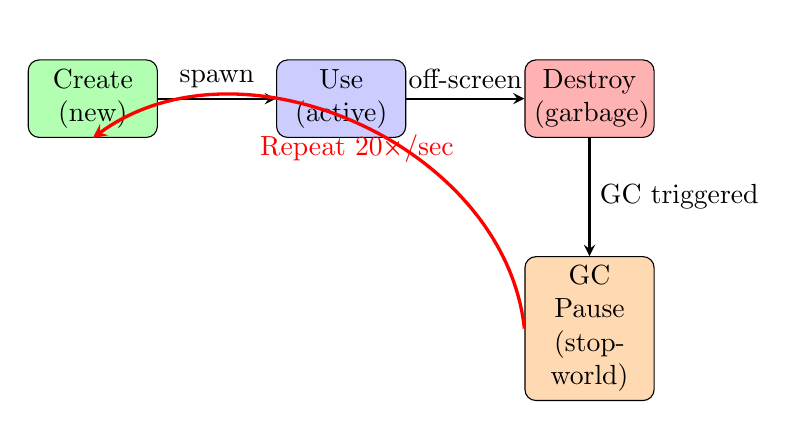
\begin{tikzpicture}[node distance=1.5cm]
            \tikzstyle{state} = [rectangle, rounded corners, draw, fill=blue!20, text width=4em, text centered, minimum height=2em]
            \tikzstyle{arrow} = [thick,->,>=stealth]

            \node [state, fill=green!30] (create) {Create\\(new)};
            \node [state, right=of create] (use) {Use\\(active)};
            \node [state, right=of use, fill=red!30] (destroy) {Destroy\\(garbage)};
            \node [state, below=of destroy, fill=orange!30] (gc) {GC Pause\\(stop-world)};

            \draw [arrow] (create) -- (use) node[midway, above] {spawn};
            \draw [arrow] (use) -- (destroy) node[midway, above] {off-screen};
            \draw [arrow] (destroy) -- (gc) node[midway, right] {GC triggered};
            \draw [arrow, bend right=60, red, very thick] (gc.west) to node[midway, below] {\textcolor{red}{Repeat 20×/sec}} (create.south);
        \end{tikzpicture}
    \end{center}

    \textbf{Problem:} Continuous allocation/deallocation cycle

    \begin{exampleblock}{Calculation (50 seconds)}
        \begin{itemize}
            \item 20 spawns/sec × 50 sec = 1000 objects created
            \item 1000 objects destroyed (off-screen removal)
            \item Result: Heavy GC workload
        \end{itemize}
    \end{exampleblock}
\end{frame}

\begin{frame}{10-03: Performance Results}
    \textbf{Actual measurements (50 seconds gameplay):}

    \begin{table}
        \centering
        \begin{tabular}{lr}
            \toprule
            \textbf{Metric} & \textbf{Value} \\
            \midrule
            Objects Created & 1000+ \\
            Objects Destroyed & 1000+ \\
            Total GC Time & 9ms \\
            GC Pauses & 2-3 minor \\
            Worst Frame & < 20ms \\
            \bottomrule
        \end{tabular}
    \end{table}

    \begin{alertblock}{Why so low?}
        Our game is small! Obstacles are tiny objects (~80 bytes each).\\
        Modern GC is efficient for small objects.
    \end{alertblock}

    \textbf{When problem becomes visible:}
    \begin{itemize}
        \item Larger objects (textures, audio, models)
        \item Higher frequency (100+ objects/second)
        \item Longer sessions (hours of gameplay)
        \item Stricter requirements (VR at 90 FPS)
    \end{itemize}
\end{frame}

\begin{frame}{10-03: Safe Spawning Algorithm}
    \textbf{Problem:} Random spawning can place obstacles in invalid positions

    \textbf{Solution:} Three-check validation

    \begin{enumerate}
        \item \textbf{Check Walkability}
        \begin{itemize}
            \item Ensure position is floor, not wall
            \item \texttt{DungeonMap.isWalkable(x, y)}
        \end{itemize}

        \item \textbf{Check Distance from NPC}
        \begin{itemize}
            \item Maintain minimum 3-tile distance
            \item Manhattan distance: $|x - npcX| + |y - npcY| \geq 3$
        \end{itemize}

        \item \textbf{Check No Overlap}
        \begin{itemize}
            \item Don't spawn on existing obstacles
            \item Loop through activeObstacles, check positions
        \end{itemize}
    \end{enumerate}

    \textbf{Max 10 attempts:} Give up if no safe position found after 10 tries
\end{frame}

% =====================================================
% SECTION 5: BRANCH 10-04 - OBJECT POOL
% =====================================================
\section{Branch 10-04: Object Pool Pattern (Solution)}

\begin{frame}{10-04: Object Pool Pattern}
    \begin{block}{Pattern Definition}
        \textbf{Intent:} Reuse expensive-to-create objects instead of creating and destroying them repeatedly.
    \end{block}

    \textbf{Key Idea:} "Borrow instead of buy"

    \begin{columns}[T]
        \begin{column}{0.48\textwidth}
            \textbf{Before (10-03):}
            \begin{itemize}
                \item Create new object
                \item Use it
                \item Destroy (becomes garbage)
                \item GC collects
                \item \textcolor{red}{Repeat 20×/sec}
            \end{itemize}
        \end{column}
        \begin{column}{0.48\textwidth}
            \textbf{After (10-04):}
            \begin{itemize}
                \item Pre-allocate pool
                \item Borrow from pool
                \item Use it
                \item Return to pool
                \item \textcolor{green}{Reuse forever!}
            \end{itemize}
        \end{column}
    \end{columns}
\end{frame}

\begin{frame}[fragile]{10-04: ObstaclePool Implementation}
    \begin{lstlisting}[basicstyle=\ttfamily\tiny]
// ObstaclePool.java
public class ObstaclePool {
    private final List<Obstacle> availableObstacles;  // Ready to borrow
    private final List<Obstacle> allObstacles;        // All pool objects
    private final ObstacleFactory factory;
    private final int maxPoolSize;

    public ObstaclePool(ObstacleFactory factory, int initialSize, int maxSize) {
        this.factory = factory;
        this.maxPoolSize = maxSize;
        this.availableObstacles = new ArrayList<>();
        this.allObstacles = new ArrayList<>();

        // Pre-allocate obstacles at startup (one-time cost!)
        for (int i = 0; i < initialSize; i++) {
            Obstacle obstacle = factory.createObstacle(0, 0);
            obstacle.setActive(false);
            availableObstacles.add(obstacle);
            allObstacles.add(obstacle);
        }
    }
    // ... acquire() and release() on next slide
}
    \end{lstlisting}
\end{frame}

\begin{frame}[fragile]{10-04: Acquire and Release}
    \begin{columns}[T]
        \begin{column}{0.48\textwidth}
            \begin{lstlisting}[basicstyle=\ttfamily\tiny]
public Obstacle acquire(int x, int y) {
    Obstacle obstacle;

    if (!availableObstacles.isEmpty()) {
        // Reuse from pool (no allocation!)
        obstacle = availableObstacles.remove(
            availableObstacles.size() - 1
        );
    } else if (allObstacles.size() < maxPoolSize) {
        // Pool empty, grow if under max
        obstacle = factory.createObstacle(x, y);
        allObstacles.add(obstacle);
    } else {
        // Pool exhausted
        return null;
    }

    obstacle.reset(x, y);  // Clean state!
    obstacle.setActive(true);
    return obstacle;
}
            \end{lstlisting}
        \end{column}
        \begin{column}{0.48\textwidth}
            \begin{lstlisting}[basicstyle=\ttfamily\tiny]
public void release(Obstacle obstacle) {
    if (obstacle == null) return;

    obstacle.setActive(false);

    if (allObstacles.contains(obstacle)
        && !availableObstacles.contains(obstacle)) {
        availableObstacles.add(obstacle);
    }
}
            \end{lstlisting}

            \vspace{0.3cm}
            \textbf{Key Points:}
            \begin{itemize}
                \item \texttt{acquire()}: Borrow from pool
                \item \texttt{reset()}: Clean state before reuse
                \item \texttt{release()}: Return to pool
                \item \textcolor{green}{No destruction!}
            \end{itemize}
        \end{column}
    \end{columns}
\end{frame}

\begin{frame}[fragile]{10-04: Reset Method (Critical!)}
    \textbf{Every reusable object MUST implement reset()}

    \begin{columns}[T]
        \begin{column}{0.48\textwidth}
            \begin{lstlisting}[basicstyle=\ttfamily\tiny]
// Obstacle.java (interface)
public interface Obstacle {
    // ... existing methods ...

    /**
     * Reset state for reuse
     * (Object Pool pattern)
     */
    void reset(int newX, int newY);
}
            \end{lstlisting}

            \begin{lstlisting}[basicstyle=\ttfamily\tiny]
// Spike.java
@Override
public void reset(int newX, int newY) {
    this.x = newX;
    this.y = newY;
    this.active = true;
    // No other state to reset
}
            \end{lstlisting}
        \end{column}
        \begin{column}{0.48\textwidth}
            \begin{lstlisting}[basicstyle=\ttfamily\tiny]
// Goblin.java
@Override
public void reset(int newX, int newY) {
    this.x = newX;
    this.y = newY;
    this.active = true;
    this.direction = 1;    // Reset direction!
    this.moveTimer = 0;    // Reset timer!
}
            \end{lstlisting}

            \begin{alertblock}{Critical!}
                \textbf{Must reset ALL mutable fields!}\\
                Forgetting a field = old state leaks into reuse
            \end{alertblock}
        \end{column}
    \end{columns}
\end{frame}

\begin{frame}[fragile]{10-04: Client Usage}
    \begin{lstlisting}[basicstyle=\ttfamily\scriptsize]
// WorldController.java (Branch 10-04)
public class WorldController {
    private List<ObstaclePool> pools;  // Pools, not factories!

    public WorldController(NPC npc) {
        this.pools = Arrays.asList(
            new ObstaclePool(new SpikeFactory(), 10, 50),
            new ObstaclePool(new GoblinFactory(), 10, 50),
            new ObstaclePool(new WolfFactory(), 10, 50)
        );
    }

    private void spawnRandomObstacle() {
        ObstaclePool pool = pools.get(random.nextInt(pools.size()));
        // ... find safe position ...

        // Borrow from pool (no new keyword!)
        Obstacle obstacle = pool.acquire(x, y);
        if (obstacle != null) {
            activeObstacles.add(obstacle);
        }
    }
}
    \end{lstlisting}

    \textcolor{green}{\textbf{acquire() instead of new!}}
\end{frame}

\begin{frame}[fragile]{10-04: Return to Pool}
    \textbf{When obstacle is no longer needed, return to pool:}

    \begin{lstlisting}[basicstyle=\ttfamily\scriptsize]
// WorldController.java
public void update(float delta) {
    // ... spawn new obstacles ...

    // Remove off-screen obstacles
    Iterator<Obstacle> iterator = activeObstacles.iterator();
    while (iterator.hasNext()) {
        Obstacle obs = iterator.next();

        if (!obs.isActive() || obs.getY() > OFF_SCREEN_Y) {
            iterator.remove();

            // Return to pool (don't destroy!)
            returnToPool(obs);
        }
    }
}

private void returnToPool(Obstacle obstacle) {
    for (ObstaclePool pool : pools) {
        if (pool.ownsObstacle(obstacle)) {
            pool.release(obstacle);
            return;
        }
    }
}
    \end{lstlisting}
\end{frame}

\begin{frame}{10-04: Object Lifecycle with Pool}
    \begin{center}
        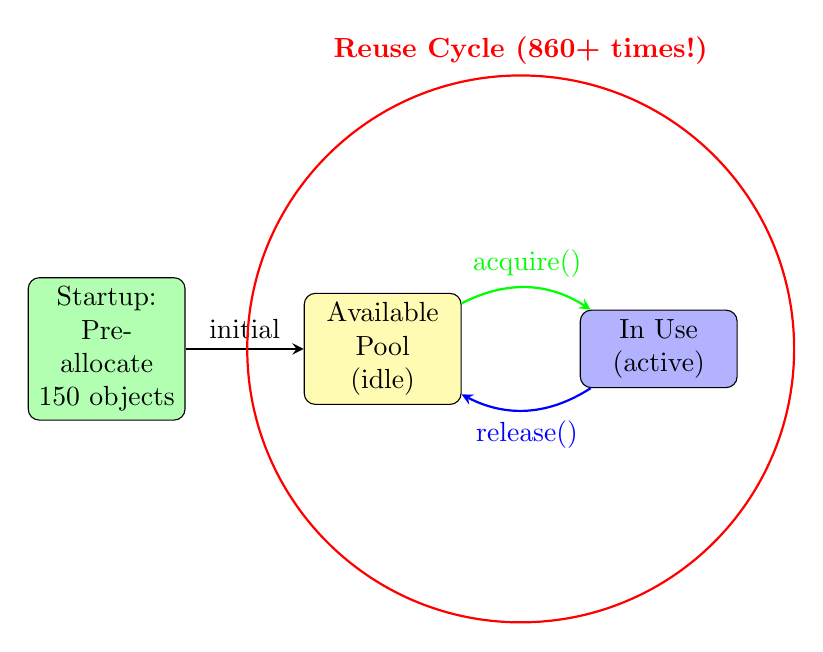
\begin{tikzpicture}[node distance=1.5cm]
            \tikzstyle{state} = [rectangle, rounded corners, draw, text width=5em, text centered, minimum height=2.5em]
            \tikzstyle{arrow} = [thick,->,>=stealth]

            \node [state, fill=green!30] (startup) {Startup:\\Pre-allocate\\150 objects};
            \node [state, right=of startup, fill=yellow!30] (available) {Available\\Pool\\(idle)};
            \node [state, right=of available, fill=blue!30] (inuse) {In Use\\(active)};

            \draw [arrow] (startup) -- (available) node[midway, above] {initial};
            \draw [arrow, bend left=30, green] (available) to node[midway, above] {acquire()} (inuse);
            \draw [arrow, bend left=30, blue] (inuse) to node[midway, below] {release()} (available);

            \node [draw=red, thick, circle, fit={(available) (inuse)}, inner sep=0.5cm, label=above:{\textcolor{red}{\textbf{Reuse Cycle (860+ times!)}}}] {};
        \end{tikzpicture}
    \end{center}

    \textbf{Key Insight:} Objects never destroyed after initial allocation!

    \begin{exampleblock}{Lifecycle Comparison}
        \textbf{10-03:} create $\rightarrow$ use $\rightarrow$ \textcolor{red}{destroy} $\rightarrow$ GC $\rightarrow$ repeat\\
        \textbf{10-04:} \textcolor{green}{pre-allocate} $\rightarrow$ acquire $\rightarrow$ use $\rightarrow$ release $\rightarrow$ \textcolor{green}{reuse}
    \end{exampleblock}
\end{frame}

\begin{frame}{10-04: Performance Results}
    \textbf{Same test (50 seconds gameplay):}

    \begin{table}
        \centering
        \begin{tabular}{lrr}
            \toprule
            \textbf{Metric} & \textbf{10-03 (No Pool)} & \textbf{10-04 (With Pool)} \\
            \midrule
            Objects Created & 1000+ & \textcolor{green}{150} \\
            Objects Destroyed & 1000+ & \textcolor{green}{0} \\
            Object Reuses & 0 & \textcolor{green}{860+} \\
            Total GC Time & 9ms & \textcolor{green}{8ms} \\
            Worst Frame & <20ms & \textcolor{green}{<18ms} \\
            \bottomrule
        \end{tabular}
    \end{table}

    \begin{block}{Key Takeaway}
        Even though GC time difference is small (9ms vs 8ms), the \textbf{pattern} matters!
        \begin{itemize}
            \item 10-03: Continuous allocation (scales badly with larger/more objects)
            \item 10-04: Zero allocation after startup (scales well!)
        \end{itemize}
    \end{block}
\end{frame}

\begin{frame}{10-04: Pool Statistics}
    \textbf{Branch 10-04 tracks pool usage:}

    \begin{lstlisting}[language=,basicstyle=\ttfamily\tiny,frame=single]
=== POOL STATISTICS ===
Spike Pool Stats:
  Total Created: 50
  Acquire Calls: 334
  Release Calls: 284
  Total Size: 50
  Available: 0
  In Use: 50

Goblin Pool Stats:
  Total Created: 50
  Acquire Calls: 334
  Release Calls: 284
  ...
    \end{lstlisting}

    \textbf{Analysis:}
    \begin{itemize}
        \item 50 created (at startup)
        \item 334 acquires = 334 times spawned
        \item 284 releases = 284 returned
        \item \textcolor{green}{\textbf{Result: 284 reuses! (85\% reuse rate)}}
    \end{itemize}
\end{frame}

% =====================================================
% SECTION 6: PATTERN COMPARISON
% =====================================================
\section{Pattern Comparison \& Trade-offs}

\begin{frame}{Factory Method vs Object Pool}
    \textbf{Different problems, different solutions!}

    \begin{table}
        \centering
        \begin{tabular}{p{4cm}p{4.5cm}p{4.5cm}}
            \toprule
            & \textbf{Factory Method} & \textbf{Object Pool} \\
            \midrule
            \textbf{Solves} & "Which TYPE to create?" & "How to REUSE objects?" \\
            \textbf{Problem} & Tight coupling, hard-coded types & GC pressure, performance \\
            \textbf{Solution} & Polymorphic creation & Object reuse \\
            \textbf{Benefit} & Extensibility, Open/Closed & Stable performance, no GC \\
            \textbf{Cost} & More classes & Higher memory, reset() complexity \\
            \bottomrule
        \end{tabular}
    \end{table}

    \begin{exampleblock}{Can Combine!}
        \textbf{Branch 10-04:} Uses BOTH patterns together\\
        Factory Method creates objects $+$ Object Pool manages their lifecycle
    \end{exampleblock}
\end{frame}

\begin{frame}{When to Use Factory Method}
    \begin{block}{Use Factory Method When:}
        \begin{itemize}
            \item ✅ Multiple polymorphic types need creation
            \item ✅ Need runtime type selection
            \item ✅ Complex initialization logic
            \item ✅ Want to decouple creation from usage
            \item ✅ System needs to be extensible (new types added)
        \end{itemize}
    \end{block}

    \begin{alertblock}{Don't Use Factory Method When:}
        \begin{itemize}
            \item ❌ Only 1-2 simple types
            \item ❌ Types never change
            \item ❌ Direct \texttt{new} is clear enough
            \item ❌ No extensibility requirements
        \end{itemize}
    \end{alertblock}

    \textbf{Rule of thumb:} If you find yourself writing switch statements for object creation, consider Factory Method!
\end{frame}

\begin{frame}{When to Use Object Pool}
    \begin{block}{Use Object Pool When:}
        \begin{itemize}
            \item ✅ High-frequency creation (>10/second)
            \item ✅ Expensive object creation (DB connections, textures)
            \item ✅ Real-time requirements (games, servers)
            \item ✅ Predictable lifetime (acquire $\rightarrow$ use $\rightarrow$ release)
            \item ✅ GC pauses are unacceptable
        \end{itemize}
    \end{block}

    \begin{alertblock}{Don't Use Object Pool When:}
        \begin{itemize}
            \item ❌ Objects created rarely (<1/second)
            \item ❌ Unpredictable lifetime
            \item ❌ Memory is constrained
            \item ❌ Objects are very simple (primitives, small structs)
            \item ❌ GC performance is acceptable
        \end{itemize}
    \end{alertblock}

    \textbf{Rule of thumb:} If GC profiler shows allocation hotspots, consider Object Pool!
\end{frame}

\begin{frame}{Trade-off: Memory vs Performance}
    \begin{columns}[T]
        \begin{column}{0.48\textwidth}
            \textbf{Without Pool (10-03):}
            \begin{itemize}
                \item \textcolor{green}{Memory efficient}
                \begin{itemize}
                    \item Only active objects in RAM
                    \item Peak: ~500 objects
                    \item Memory fluctuates
                \end{itemize}
                \item \textcolor{red}{Performance variable}
                \begin{itemize}
                    \item GC pauses unpredictable
                    \item Frame times fluctuate
                    \item Allocation overhead
                \end{itemize}
            \end{itemize}
        \end{column}
        \begin{column}{0.48\textwidth}
            \textbf{With Pool (10-04):}
            \begin{itemize}
                \item \textcolor{red}{Higher memory usage}
                \begin{itemize}
                    \item All pool objects in RAM
                    \item Fixed: 150 objects
                    \item Memory constant
                \end{itemize}
                \item \textcolor{green}{Performance predictable}
                \begin{itemize}
                    \item Minimal GC
                    \item Stable frame times
                    \item No allocation overhead
                \end{itemize}
            \end{itemize}
        \end{column}
    \end{columns}

    \vspace{0.5cm}
    \begin{exampleblock}{Design Decision}
        \textbf{Games:} Usually prefer predictable performance (pooling)\\
        \textbf{Mobile/Embedded:} May prefer memory efficiency (no pooling)
    \end{exampleblock}
\end{frame}

\begin{frame}{Alternative Patterns}
    \textbf{Other creational patterns to consider:}

    \begin{enumerate}
        \item \textbf{Abstract Factory}
        \begin{itemize}
            \item Creates \textit{families} of related objects
            \item Example: EasyModeFactory vs HardModeFactory
            \item When: Need themed object sets
        \end{itemize}

        \item \textbf{Builder}
        \begin{itemize}
            \item Step-by-step object construction
            \item Example: \texttt{new ObstacleBuilder().at(10,10).withDamage(30).build()}
            \item When: Many optional parameters
        \end{itemize}

        \item \textbf{Prototype}
        \begin{itemize}
            \item Clone existing objects
            \item Example: \texttt{prototype.clone().setPosition(x, y)}
            \item When: Cloning cheaper than creating
        \end{itemize}
    \end{enumerate}

    \textbf{Choose pattern based on specific problem!}
\end{frame}

% =====================================================
% SECTION 7: PRACTICAL APPLICATION
% =====================================================
\section{Practical Application}

\begin{frame}{Real-World Examples}
    \textbf{Where these patterns are used professionally:}

    \begin{block}{Factory Method in the Wild}
        \begin{itemize}
            \item \textbf{Unity:} Prefab instantiation, Component factories
            \item \textbf{Spring Framework:} BeanFactory for dependency injection
            \item \textbf{JDBC:} DriverManager.getConnection() creates database connections
            \item \textbf{Unreal Engine:} SpawnActor<T>() factory method
        \end{itemize}
    \end{block}

    \begin{block}{Object Pool in the Wild}
        \begin{itemize}
            \item \textbf{Unity:} ObjectPool<T> for bullets, particles, enemies
            \item \textbf{Apache Commons:} GenericObjectPool for DB connections
            \item \textbf{Game Engines:} Particle systems, VFX pools
            \item \textbf{Web Servers:} Thread pools (Tomcat, Jetty)
            \item \textbf{Networking:} Buffer pools, socket pools
        \end{itemize}
    \end{block}
\end{frame}

\begin{frame}{Case Study: Unity's ObjectPool<T>}
    \textbf{Unity provides built-in object pooling since 2021}

    \begin{columns}[T]
        \begin{column}{0.48\textwidth}
            \textbf{Before (Manual):}
            \begin{itemize}
                \item Instantiate(bulletPrefab)
                \item Destroy(bullet)
                \item GC pressure in large games
                \item Visible stuttering
            \end{itemize}
        \end{column}
        \begin{column}{0.48\textwidth}
            \textbf{After (ObjectPool):}
            \begin{itemize}
                \item pool.Get()
                \item pool.Release(bullet)
                \item Zero GC from bullets
                \item Smooth gameplay
            \end{itemize}
        \end{column}
    \end{columns}

    \vspace{0.3cm}
    \textbf{Performance Impact (Unity shooter game):}
    \begin{itemize}
        \item Without pool: 100+ bullets/sec = 50ms GC spike every 5 seconds
        \item With pool: Zero GC from bullets, stable 60 FPS
    \end{itemize}

    \begin{exampleblock}{Industry Standard}
        Major games (Fortnite, Gears of War, etc.) use extensive object pooling
    \end{exampleblock}
\end{frame}

\begin{frame}{Performance Profiling Tips}
    \textbf{How to identify if you need object pooling:}

    \begin{enumerate}
        \item \textbf{Use Profiler}
        \begin{itemize}
            \item Java: visualvm, JProfiler, YourKit
            \item Unity: Unity Profiler
            \item Look for allocation hotspots
        \end{itemize}

        \item \textbf{Monitor GC}
        \begin{itemize}
            \item Java: \texttt{-Xlog:gc*} flag
            \item Check GC pause frequency and duration
            \item Look for young generation collections
        \end{itemize}

        \item \textbf{Measure Frame Times}
        \begin{itemize}
            \item Track min/max/average frame time
            \item Identify frame drops
            \item Correlate with GC events
        \end{itemize}
    \end{enumerate}

    \begin{alertblock}{Golden Rule}
        \textit{"Profile first, optimize second"}\\
        Don't apply pooling everywhere - only where measurements show it helps!
    \end{alertblock}
\end{frame}

\begin{frame}{Common Pitfalls}
    \textbf{Mistakes to avoid:}

    \begin{enumerate}
        \item \textbf{Forgot to call reset()}
        \begin{itemize}
            \item Symptom: Object has old state from previous use
            \item Solution: Always call \texttt{reset()} in \texttt{acquire()}
        \end{itemize}

        \item \textbf{Incomplete reset() implementation}
        \begin{itemize}
            \item Symptom: Some fields keep old values
            \item Solution: Reset ALL mutable fields, not just position
        \end{itemize}

        \item \textbf{Pool too small (exhaustion)}
        \begin{itemize}
            \item Symptom: \texttt{acquire()} returns null
            \item Solution: Increase pool size or implement growth
        \end{itemize}

        \item \textbf{Forgot to release()}
        \begin{itemize}
            \item Symptom: Pool gradually empties, performance degrades
            \item Solution: Always pair \texttt{acquire()} with \texttt{release()}
        \end{itemize}
    \end{enumerate}
\end{frame}

\begin{frame}{Testing Pooled Objects}
    \textbf{How to test object pooling:}

    \begin{block}{Unit Tests}
        \begin{enumerate}
            \item Test acquire from full pool
            \item Test acquire from empty pool (growth)
            \item Test release returns to pool
            \item \textbf{Test reset cleans ALL state}
        \end{enumerate}
    \end{block}

    \textbf{Example: Test reset():}
    \begin{verbatim}
@Test
void testResetCleansState() {
    ObstaclePool pool = new ObstaclePool(new GoblinFactory(), 1, 1);
    Obstacle obs1 = pool.acquire(10, 10);
    obs1.setActive(false);
    pool.release(obs1);

    Obstacle obs2 = pool.acquire(20, 20);
    assertTrue(obs2.isActive());  // Should be reset!
    assertEquals(20, obs2.getX());
}
    \end{verbatim}
\end{frame}

% =====================================================
% SECTION 8: DESIGN PRINCIPLES
% =====================================================
\section{Design Principles Review}

\begin{frame}{SOLID Principles Applied}
    \textbf{Week 10 demonstrates multiple SOLID principles:}

    \begin{block}{Open/Closed Principle (Factory Method)}
        \textit{"Open for extension, closed for modification"}
        \begin{itemize}
            \item Can add new obstacle types without modifying WorldController
            \item Just create new factory and register it
            \item No risk of breaking existing code
        \end{itemize}
    \end{block}

    \begin{block}{Single Responsibility Principle}
        \begin{itemize}
            \item \textbf{Factory:} Responsible for creation only
            \item \textbf{Pool:} Responsible for lifecycle management only
            \item \textbf{Obstacle:} Responsible for behavior only
            \item \textbf{WorldController:} Responsible for game logic only
        \end{itemize}
    \end{block}
\end{frame}

\begin{frame}{Dependency Inversion Principle}
    \begin{block}{Principle}
        \textit{"Depend on abstractions, not concretions"}
    \end{block}

    \textbf{Applied in Branch 10-02:}

    \begin{center}
        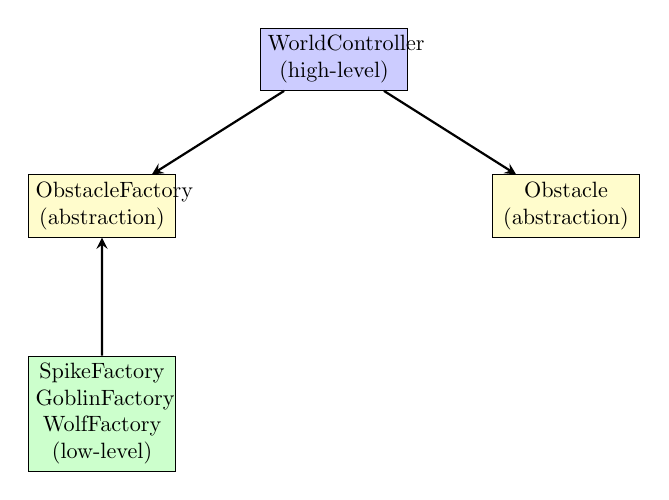
\begin{tikzpicture}[node distance=1.5cm, scale=0.8, every node/.style={scale=0.8}]
            \tikzstyle{class} = [rectangle, draw, text width=6em, text centered, minimum height=2em]
            \tikzstyle{interface} = [rectangle, draw, fill=yellow!20, text width=6em, text centered]
            \tikzstyle{arrow} = [thick,->,>=stealth]

            \node [class, fill=blue!20] (wc) {WorldController\\(high-level)};
            \node [interface, below left=of wc] (factory) {ObstacleFactory\\(abstraction)};
            \node [interface, below right=of wc] (obs) {Obstacle\\(abstraction)};
            \node [class, fill=green!20, below=of factory] (concrete) {SpikeFactory\\GoblinFactory\\WolfFactory\\(low-level)};

            \draw [arrow] (wc) -- (factory);
            \draw [arrow] (wc) -- (obs);
            \draw [arrow] (concrete) -- (factory);
        \end{tikzpicture}
    \end{center}

    \textbf{High-level module (WorldController) does NOT depend on low-level modules (concrete factories)!}
\end{frame}

\begin{frame}{Separation of Concerns}
    \textbf{Week 10 continues separation of concerns from Week 9:}

    \begin{columns}[T]
        \begin{column}{0.48\textwidth}
            \textbf{Week 9:}
            \begin{itemize}
                \item Separate update from render
                \item Separate logic from display
                \item Centralize global state
            \end{itemize}
        \end{column}
        \begin{column}{0.48\textwidth}
            \textbf{Week 10:}
            \begin{itemize}
                \item Separate creation from usage
                \item Separate lifecycle from behavior
                \item Separate type selection from instantiation
            \end{itemize}
        \end{column}
    \end{columns}

    \vspace{0.5cm}
    \begin{exampleblock}{Progressive Refinement}
        Each week adds new layer of architectural sophistication:
        \begin{itemize}
            \item Week 9: Fix structure and performance basics
            \item Week 10: Fix extensibility and memory management
            \item Future: Advanced patterns (Strategy, Observer, Command, State)
        \end{itemize}
    \end{exampleblock}
\end{frame}

% =====================================================
% SECTION 9: EXERCISES
% =====================================================
\section{Practice Exercises}

\begin{frame}{Exercise 1: Add Trap Factory (Easy)}
    \textbf{Task:} Add a Trap obstacle using Factory Method pattern

    \textbf{Requirements:}
    \begin{itemize}
        \item Create \texttt{Trap.java} implementing Obstacle interface
        \item Damage = 15 HP, Symbol = 'T'
        \item Static (doesn't move)
        \item Deactivates after first hit
        \item Create \texttt{TrapFactory.java}
        \item Register in WorldController factories list
    \end{itemize}

    \textbf{Learning Outcomes:}
    \begin{itemize}
        \item Practice Factory Method pattern
        \item Understand polymorphic creation
        \item Test extensibility without modifying existing code
    \end{itemize}

    \textbf{Verification:} Run game, observe Trap spawning, test collision
\end{frame}

\begin{frame}{Exercise 2: PowerUp Pool (Medium)}
    \textbf{Task:} Implement HealthPack power-up with object pooling

    \textbf{Requirements:}
    \begin{itemize}
        \item Create \texttt{HealthPack.java} with \texttt{reset()} method
        \item Heals +20 HP (don't exceed max)
        \item Symbol = 'H'
        \item Create \texttt{HealthPackFactory.java}
        \item Create \texttt{HealthPackPool.java}
        \item Pool size = 5 objects
        \item Respawn every 5 seconds
    \end{itemize}

    \textbf{Challenges:}
    \begin{itemize}
        \item How to handle respawn timing?
        \item Should respawn use pool or create new?
        \item What if all 5 HealthPacks are active?
    \end{itemize}
\end{frame}

\begin{frame}{Exercise 3: Performance Comparison (Medium)}
    \textbf{Task:} Measure and compare GC performance

    \textbf{Steps:}
    \begin{enumerate}
        \item Run branch 10-03 for 10 minutes
        \item Collect metrics (GC time, pauses, worst frame)
        \item Run branch 10-04 for 10 minutes
        \item Collect same metrics
        \item Create comparison chart (Excel/Python)
        \item Write report analyzing differences
    \end{enumerate}

    \textbf{Learning Outcomes:}
    \begin{itemize}
        \item Performance measurement techniques
        \item Understanding GC impact over time
        \item Data visualization skills
    \end{itemize}

    \textbf{Tools:} PerformanceMonitor output, visualvm (optional)
\end{frame}

\begin{frame}{Exercise 4: Boss with Minion Factory (Hard)}
    \textbf{Task:} Create Boss enemy that spawns minions

    \textbf{Requirements:}
    \begin{itemize}
        \item \texttt{Boss.java}: Large HP (100), spawns Goblins every 3 seconds
        \item \texttt{BossFactory.java}: Creates Boss with reference to GoblinFactory
        \item Boss uses GoblinFactory to spawn minions
        \item Minions should use object pool for performance
        \item Track Boss' minions for cleanup when Boss dies
    \end{itemize}

    \textbf{Design Challenges:}
    \begin{itemize}
        \item How to pass GoblinFactory to Boss?
        \item Should minions be pooled separately?
        \item How to prevent spawning when pool exhausted?
        \item How to ensure minions released when Boss dies?
    \end{itemize}

    \textbf{Learning:} Composition of patterns, complex object relationships
\end{frame}

% =====================================================
% SECTION 10: SUMMARY
% =====================================================
\section{Summary}

\begin{frame}{Key Takeaways}
    \begin{enumerate}
        \item \textbf{Patterns Solve Specific Problems}
        \begin{itemize}
            \item Factory Method: Extensible object creation
            \item Object Pool: Performance through reuse
            \item Don't use patterns "just because"
        \end{itemize}

        \item \textbf{Trade-offs Matter}
        \begin{itemize}
            \item Factory: More classes vs better structure
            \item Pool: Memory vs performance
            \item Choose based on requirements
        \end{itemize}

        \item \textbf{Patterns Can Combine}
        \begin{itemize}
            \item Branch 10-04 uses Factory + Pool together
            \item Factory creates initial pool objects
            \item Pool manages their lifecycle
        \end{itemize}
    \end{enumerate}
\end{frame}

\begin{frame}{Week 10 Evolution Summary}
    \begin{center}
        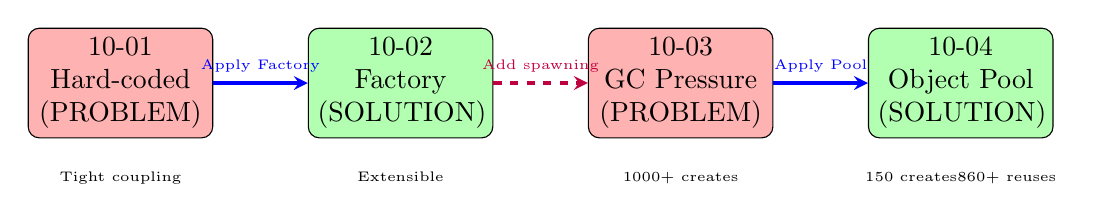
\begin{tikzpicture}[node distance=1.2cm]
            \tikzstyle{branch} = [rectangle, rounded corners, draw, text width=6em, text centered, minimum height=2.5em]
            \tikzstyle{arrow} = [thick,->,>=stealth]

            \node [branch, fill=red!30] (b1) {10-01\\Hard-coded\\(PROBLEM)};
            \node [branch, fill=green!30, right=of b1] (b2) {10-02\\Factory\\(SOLUTION)};
            \node [branch, fill=red!30, right=of b2] (b3) {10-03\\GC Pressure\\(PROBLEM)};
            \node [branch, fill=green!30, right=of b3] (b4) {10-04\\Object Pool\\(SOLUTION)};

            \draw [arrow, blue, very thick] (b1) -- (b2) node[midway, above] {\tiny Apply Factory};
            \draw [arrow, purple, very thick, dashed] (b2) -- (b3) node[midway, above] {\tiny Add spawning};
            \draw [arrow, blue, very thick] (b3) -- (b4) node[midway, above] {\tiny Apply Pool};

            \node [below=0.3cm of b1] {\tiny Tight coupling};
            \node [below=0.3cm of b2] {\tiny Extensible};
            \node [below=0.3cm of b3] {\tiny 1000+ creates};
            \node [below=0.3cm of b4] {\tiny 150 creates\\860+ reuses};
        \end{tikzpicture}
    \end{center}

    \begin{block}{Progressive Problem-Solving}
        Each branch builds on previous:
        \begin{itemize}
            \item Identify problem $\rightarrow$ Apply pattern $\rightarrow$ New problem emerges $\rightarrow$ Apply new pattern
            \item Real software development: iterative refinement
        \end{itemize}
    \end{block}
\end{frame}

\begin{frame}{Design Principles Review}
    \textbf{Week 10 demonstrates:}

    \begin{itemize}
        \item ✅ \textbf{Open/Closed Principle:} Extend with new factories without modifying WorldController
        \item ✅ \textbf{Single Responsibility:} Factory creates, Pool manages, Obstacle behaves
        \item ✅ \textbf{Dependency Inversion:} Depend on ObstacleFactory interface, not concrete classes
        \item ✅ \textbf{Separation of Concerns:} Creation logic separate from usage logic
        \item ✅ \textbf{Don't Repeat Yourself:} One factory per type, reusable across game
    \end{itemize}

    \vspace{0.5cm}
    \begin{exampleblock}{Industry Relevance}
        These patterns are used in every major game engine:
        \begin{itemize}
            \item Unity: ObjectPool<T>, Prefab factories
            \item Unreal: SpawnActor factories, object pooling systems
            \item Professional games: Extensive use of both patterns
        \end{itemize}
    \end{exampleblock}
\end{frame}

\begin{frame}{Further Learning}
    \textbf{Recommended Resources:}

    \begin{block}{Books}
        \begin{itemize}
            \item \textbf{"Game Programming Patterns"} by Robert Nystrom (FREE online!)
            \item \textbf{"Design Patterns"} by Gang of Four (classic)
            \item \textbf{"Head First Design Patterns"} (beginner-friendly)
        \end{itemize}
    \end{block}

    \begin{block}{Online}
        \begin{itemize}
            \item Unity Learn: Object Pooling tutorial
            \item Refactoring.Guru: Visual pattern explanations
            \item GitHub: Our complete Week 10 repository
        \end{itemize}
    \end{block}

    \begin{block}{Practice}
        \begin{itemize}
            \item Complete all 4 exercises
            \item Refactor your own projects
            \item Build a small game using these patterns
        \end{itemize}
    \end{block}
\end{frame}

\begin{frame}{Next Steps}
    \textbf{Future Topics (Week 11+):}

    \begin{enumerate}
        \item \textbf{Behavioral Patterns}
        \begin{itemize}
            \item Strategy: Interchangeable AI behaviors
            \item Observer: Event-driven systems
            \item Command: Undo/redo, input buffering
            \item State Machine: Complex entity behaviors
        \end{itemize}

        \item \textbf{Advanced Game Architecture}
        \begin{itemize}
            \item Entity-Component-System (ECS)
            \item Update methods (game loop patterns)
            \item Service Locator for game services
        \end{itemize}

        \item \textbf{Performance Optimization}
        \begin{itemize}
            \item Spatial hashing for collision detection
            \item Dirty flag pattern
            \item Data locality and cache efficiency
        \end{itemize}
    \end{enumerate}
\end{frame}

% =====================================================
% FINAL SLIDE
% =====================================================
\begin{frame}{Thank You!}
    \begin{center}
        \Huge\textbf{Questions?}

        \vspace{1cm}
        \Large Week 10: Factory Method \& Object Pool

        \vspace{0.5cm}
        \normalsize
        \textbf{Repository:} \texttt{github.com/yourrepo/oop-rpg}\\
        \textbf{Documentation:} \texttt{docs/week-10-overview.md}\\
        \textbf{Analysis:} \texttt{docs/10-05-analysis.md}

        \vspace{1cm}
        \textit{Next week: Behavioral Patterns (Strategy \& Observer)}
    \end{center}
\end{frame}

\end{document}
